\section{Overview}

Before explaining the main parts of GIMMIX, this section gives an overview and introduces the basic components, that are used throughout the code.

Conceptually, GIMMIX consists of several \i{modules} that interact with each other. The name of a module corresponds to a source file or folder in the directory \file{src} and to the associated header file or folder in the directory \file{include}. The following \gls{FMC} diagram illustrates the most important modules and their relationships, whereas the CLI, the core and the devices are only shown as black boxes for now:
\begin{figure}[H]
	\centering
	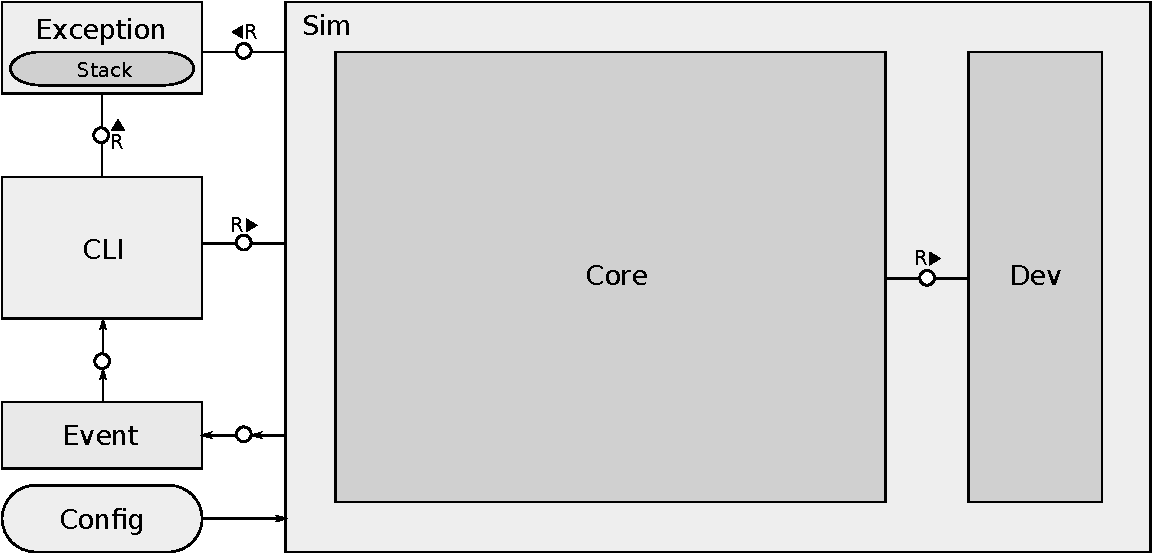
\includegraphics[width=\textwidth]{img/sim-fmc-crop.pdf}
	\caption{Architecture of GIMMIX in \protect\gls{FMC} notation}
	\label{fig:gimmix-arch}
\end{figure}
\noindent That means, the modules \i{core} and \i{dev}, to which the core sends requests for tasks like reading an octa from a specific physical address, are in a sense enveloped in \i{sim}. Sim supports some basic operations like initializing the whole system, resetting it or shutting it down. This is controlled by the module \i{CLI} (when running in interactive mode). The following sections describe the other general modules in the figure.

\subsection{Exception}

Although \glslink{Exception}{exception} handling in C via `setjmp` and `longjmp` is not as convenient and powerful as for example in Java, it offers some advantages. That is, it separates "normal" code from exceptional code and provides the possibility to handle an \glslink{Exception}{exception} only at places, where it can be handled in a sensible way. To achieve that and allow nested "try and catches", the module \i{exception} manages a stack of `jmp_buf`s, which hold the state created by `setjmp`. It is used for trips and traps in the core and also for \glslink{Exception}{exceptions} in the CLI. The most important functions are:
\begin{itemize}
	\item `ex_push(jmp_buf *environment)`:\\
	This function pushes the given environment onto the stack and is thus the equivalent to a `try`. The environment \i{has to} be created by the caller, because one can not jump back to a stack frame, that has been already destroyed.
	\item `ex_throw(int exception,octa bits)`:\\
	As the name suggests, it throws the \glslink{Exception}{exception} with given number and additional information in `bits`, which is used for example to specify what trip or trap should be triggered. That is, it calls `longjmp` with the topmost `jmpbuf` and `exception` as arguments, so that the caller of `setjmp` receives `exception` as return-value.
	\item `ex_pop()`:\\
	This function removes the topmost environment from the stack. Hence, it is the equivalent to the end of a try-catch-construct.
\end{itemize}
In this thesis, the term "\glslink{Exception}{exception}" without the prefix "arithmetical", "program" or "machine", refers to this concept, instead of the different \glslink{Exception}{exceptions} of MMIX.

\subsection{Event}

As already mentioned, GIMMIX offers a sophisticated CLI that should allow it to debug an operating system or other programs in a convenient way. To do so, the CLI needs of course access to the core, \ie it has to read the current state and should also be able to display the effect of an instruction or set breakpoints. Integrating all those facilities into the core would mean, that it gets more difficult to read and understand and it would also introduce strong coupling between the CLI and the core. Since the core is quite stable (the architecture is not expected to change much), but it may indeed be imaginable to provide a graphical user interface (GUI) to GIMMIX some day, it has been decided to work with events to supply the user interface with information. This way, the core is completely independent of the CLI and thus, assuming that a GUI is ready, it could replace the CLI within minutes, without affecting the core.

The module \i{event} implements this idea by providing `ev_register` to register a callback function for a specific event and `ev_unregister` to unregister it again. Additionally, events can be fired by calling `ev_fire`, `ev_fire1` or `ev_fire2` to raise an event with 0, 1 or 2 arguments, respectively. As figure \ref{fig:gimmix-arch} suggests, the core fires events and the event module forwards them to the CLI (and any other interested modules), which has registered the corresponding callbacks at the beginning. It is noteworthy, that if GIMMIX is used in non-interactive mode, the CLI will not be used at all and thus no callback will be registered, which will allow GIMMIX to be as performant as possible.

\subsection{Config}

Of course, GIMMIX should be configurable to some extent, which is realized by the module \i{config}. It consists of two categories of settings: the settings in the first one are configurable during compile time (\ie constants are used) and the other ones are configurable during runtime. The latter can be passed to GIMMIX as command line arguments. In a sense, the compile time options are those that would be fixed when GIMMIX were a solid piece of hardware (number of local registers, cache size, device addresses, \dots), while the runtime options could be changed more easily (amount of main memory, number of terminals, disk image, \dots). But of course, there are also practical reasons, why one has to be able to specify the disk image or the rom image via command line argument.

